\documentclass{article}\usepackage[]{graphicx}\usepackage[]{xcolor}
% maxwidth is the original width if it is less than linewidth
% otherwise use linewidth (to make sure the graphics do not exceed the margin)
\makeatletter
\def\maxwidth{ %
  \ifdim\Gin@nat@width>\linewidth
    \linewidth
  \else
    \Gin@nat@width
  \fi
}
\makeatother

\definecolor{fgcolor}{rgb}{0.345, 0.345, 0.345}
\newcommand{\hlnum}[1]{\textcolor[rgb]{0.686,0.059,0.569}{#1}}%
\newcommand{\hlsng}[1]{\textcolor[rgb]{0.192,0.494,0.8}{#1}}%
\newcommand{\hlcom}[1]{\textcolor[rgb]{0.678,0.584,0.686}{\textit{#1}}}%
\newcommand{\hlopt}[1]{\textcolor[rgb]{0,0,0}{#1}}%
\newcommand{\hldef}[1]{\textcolor[rgb]{0.345,0.345,0.345}{#1}}%
\newcommand{\hlkwa}[1]{\textcolor[rgb]{0.161,0.373,0.58}{\textbf{#1}}}%
\newcommand{\hlkwb}[1]{\textcolor[rgb]{0.69,0.353,0.396}{#1}}%
\newcommand{\hlkwc}[1]{\textcolor[rgb]{0.333,0.667,0.333}{#1}}%
\newcommand{\hlkwd}[1]{\textcolor[rgb]{0.737,0.353,0.396}{\textbf{#1}}}%
\let\hlipl\hlkwb

\usepackage{framed}
\makeatletter
\newenvironment{kframe}{%
 \def\at@end@of@kframe{}%
 \ifinner\ifhmode%
  \def\at@end@of@kframe{\end{minipage}}%
  \begin{minipage}{\columnwidth}%
 \fi\fi%
 \def\FrameCommand##1{\hskip\@totalleftmargin \hskip-\fboxsep
 \colorbox{shadecolor}{##1}\hskip-\fboxsep
     % There is no \\@totalrightmargin, so:
     \hskip-\linewidth \hskip-\@totalleftmargin \hskip\columnwidth}%
 \MakeFramed {\advance\hsize-\width
   \@totalleftmargin\z@ \linewidth\hsize
   \@setminipage}}%
 {\par\unskip\endMakeFramed%
 \at@end@of@kframe}
\makeatother

\definecolor{shadecolor}{rgb}{.97, .97, .97}
\definecolor{messagecolor}{rgb}{0, 0, 0}
\definecolor{warningcolor}{rgb}{1, 0, 1}
\definecolor{errorcolor}{rgb}{1, 0, 0}
\newenvironment{knitrout}{}{} % an empty environment to be redefined in TeX

\usepackage{alltt}
\usepackage{amsmath} %This allows me to use the align functionality.
                     %If you find yourself trying to replicate
                     %something you found online, ensure you're
                     %loading the necessary packages!
\usepackage{amsfonts}%Math font
\usepackage{graphicx}%For including graphics
\usepackage{hyperref}%For Hyperlinks
\usepackage[shortlabels]{enumitem}% For enumerated lists with labels specified
                                  % We had to run tlmgr_install("enumitem") in R
\hypersetup{colorlinks = true,citecolor=black} %set citations to have black (not green) color
\usepackage{natbib}        %For the bibliography
\setlength{\bibsep}{0pt plus 0.3ex}
\bibliographystyle{apalike}%For the bibliography
\usepackage[margin=0.50in]{geometry}
\usepackage{float}
\usepackage{multicol}

%fix for figures
\usepackage{caption}
\newenvironment{Figure}
  {\par\medskip\noindent\minipage{\linewidth}}
  {\endminipage\par\medskip}
\IfFileExists{upquote.sty}{\usepackage{upquote}}{}
\begin{document}

\vspace{-1in}
\title{Lab 8 -- MATH 240 -- Computational Statistics}

\author{
  Avery Johnson \\
  Colgate University  \\
  Department of Mathematics  \\
  {\tt aqjohnson@colgate.edu}
}

\date{}

\maketitle

\begin{multicols}{2}
\begin{abstract}
The Beta distribution is a flexible probability distribution defined on the interval (0,1), often used to model proportions and probabilities. This lab investigates the properties of the Beta distribution, including its mean, variance, skewness, and kurtosis, using both theoretical derivations and numerical simulations. Through the generation of Beta-distributed samples, the convergence of sample statistics to population values is examined, highlighting the importance of sample size in statistical examination. Additionally, two estimation methods, the Method of Moments (MOM) and Maximum Likelihood Estimation (MLE), are compared using simulated real-world data. The effectiveness of these methods is evaluated through repeated sampling, with results demonstrating that the MLE provides more accurate and precise estimates than MOM. The application of the Beta distribution to country death rate data further illustrates its relevance in real-world modeling. 

\end{abstract}

\noindent \textbf{Keywords:} 
Beta distribution, moments, mean, variance, skewness, kurtosis, MOM estimator, MLE estimator.

\section{Introduction}
The Beta distribution is a continuous probability distribution defined on $[0,1]$. It is commonly used to model proportions, probabilities, and rates, making it useful in a variety of statistical and real-world applications. The shape of the Beta distribution is controlled by two parameters, $\alpha$ and $\beta$, which determine its skewness and characteristics. This lab explores the properties of the Beta distribution, compares theoretical and sample-based estimates, and applies parameter estimation techniques to real-world data. The primary objectives are to analyze the Beta distribution's properties, to compare sample statistics with true population values, to estimate the parameters $\alpha$ and $\beta$ from real-world data using the Method of Moments (MLE) and Maximum Likelihood Estimation (MLE), and to assess the effectiveness of different estimation techniques using simulation.

\section{Density Functions and Parameters}
The probability density function (PDF) of a beta distribution is given by:

$$
f_X(x \mid \alpha, \beta) = \frac{\Gamma(\alpha + \beta)}{\Gamma \alpha \Gamma \beta} x^{\alpha-1} (1-x)^{\beta - 1} I(x \in [0,1])
$$
where $I(x \in [0,1]) = 1$ when $x \in [0, 1]$ and $0$ otherwise.

To visualize the impact of the parameters $\alpha$ and $\beta$ on the distribution, four cases were examined: Beta(2,5), Beta(5,5), Beta(5,2), and Beta(0.5,0.5). The first distribution is right-skewed, the second is symmetric, the third is left-skewed, and the forth is U-shaped. These distributions were plotted to illustrate how the parameters influence the shape of the density function. The plots in Figure \ref{populationfigures} demonstrate that increasing $\alpha$ shifts the distribution towards 1, while increasing $\beta$ shifts it towards zero. When $\alpha = \beta$, the distribution is symmetric. 


\section{Properties}
The Beta distribution's key properties include its mean, variance, skewness, and kurtosis. Each of the properties relies on $\alpha$ and $\beta$, showing how the distribution's shape and behavior changes depending on the parameters. These moments were computed using numerical integration and verified against the theoretical values in Table \ref{populationsummary}. 
To evaluate whether data summaries of random samples connect to the actual population distribution, random samples of size 500 were drawn from each Beta distribution. The sample mean, variance, skewness, and kurtosis were computed as can be seen in Table \ref{samplestatistics}. These were then compared to population-level quantities in Table \ref{populationsummary}, and we conclude that the values closely resembled one another. Furthermore, the histograms and estimated density in Figure \ref{samplehistograms} demonstrate that the samples, in each case, closely resemble the theoretical Beta probability density functions. From this analysis, we confirmed that both our graphical and numerical summaries of random samples connect to the actual population distribution.



% latex table generated in R 4.4.2 by xtable 1.8-4 package
% Tue Mar 25 22:35:30 2025
\begin{table}[H]
\centering
\begingroup\small
\begin{tabular}{rrrrrr}
  \hline
alpha & beta & mean & var & skew & kurtosis \\ 
  \hline
2.00 & 5.00 & 0.29 & 0.03 & 0.60 & -0.12 \\ 
  5.00 & 5.00 & 0.50 & 0.02 & 0.00 & -0.46 \\ 
  5.00 & 2.00 & 0.71 & 0.03 & -0.60 & -0.12 \\ 
  0.50 & 0.50 & 0.50 & 0.12 & 0.00 & -1.50 \\ 
   \hline
\end{tabular}
\endgroup
\caption{Population-Level Summary} 
\label{populationsummary}
\end{table}


% latex table generated in R 4.4.2 by xtable 1.8-4 package
% Tue Mar 25 22:35:30 2025
\begin{table}[H]
\centering
\begingroup\small
\begin{tabular}{rrrrrr}
  \hline
alpha & beta & mean & var & skew & kurtosis \\ 
  \hline
2.00 & 5.00 & 0.29 & 0.03 & 0.57 & -0.23 \\ 
  5.00 & 5.00 & 0.50 & 0.02 & -0.06 & -0.58 \\ 
  5.00 & 2.00 & 0.71 & 0.03 & -0.57 & -0.23 \\ 
  0.50 & 0.50 & 0.51 & 0.13 & -0.02 & -1.51 \\ 
   \hline
\end{tabular}
\endgroup
\caption{Sample Summary} 
\label{samplestatistics}
\end{table}


\section{Estimators}


\section{Death Rates Example}


%%%%%%%%%%%%%%%%%%%%%%%%%%%%%%%%%%%%%%%%%%%%%%%%%%%%%%%%%%%%%%%%%%%%%%%%%%%%%%%%
% Bibliography
%%%%%%%%%%%%%%%%%%%%%%%%%%%%%%%%%%%%%%%%%%%%%%%%%%%%%%%%%%%%%%%%%%%%%%%%%%%%%%%%
\vspace{2em}

\noindent\textbf{Bibliography:} 

\begin{tiny}
\bibliography{bib}
\end{tiny}


\end{multicols}

%%%%%%%%%%%%%%%%%%%%%%%%%%%%%%%%%%%%%%%%%%%%%%%%%%%%%%%%%%%%%%%%%%%%%%%%%%%%%%%%
% Appendix
%%%%%%%%%%%%%%%%%%%%%%%%%%%%%%%%%%%%%%%%%%%%%%%%%%%%%%%%%%%%%%%%%%%%%%%%%%%%%%%%
\newpage
\onecolumn
\section{Appendix}

\subsection{Density Function and Parameters}
\subsubsection{Population Distribution Figures}
\begin{knitrout}\scriptsize
\definecolor{shadecolor}{rgb}{0.969, 0.969, 0.969}\color{fgcolor}
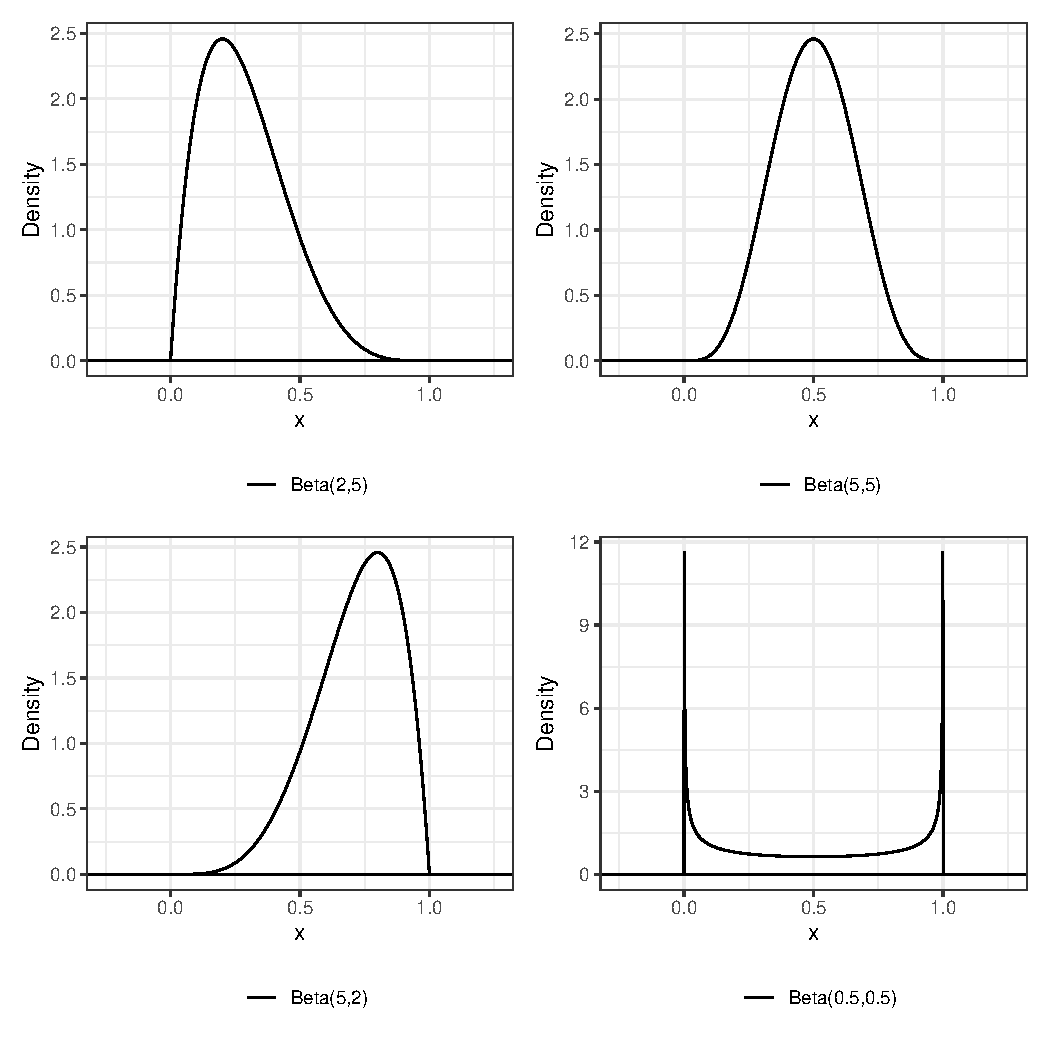
\includegraphics[width=\maxwidth]{figure/plot1-1} 
\end{knitrout}

\begin{figure}[H]
\begin{center}

\caption{Population Figures for Various Beta Distributions}
\label{populationfigures} %we can now reference plot1
\end{center}
\end{figure}

\subsection{Properties}
\subsubsection{Sample Distribution Figures}
\begin{knitrout}\scriptsize
\definecolor{shadecolor}{rgb}{0.969, 0.969, 0.969}\color{fgcolor}
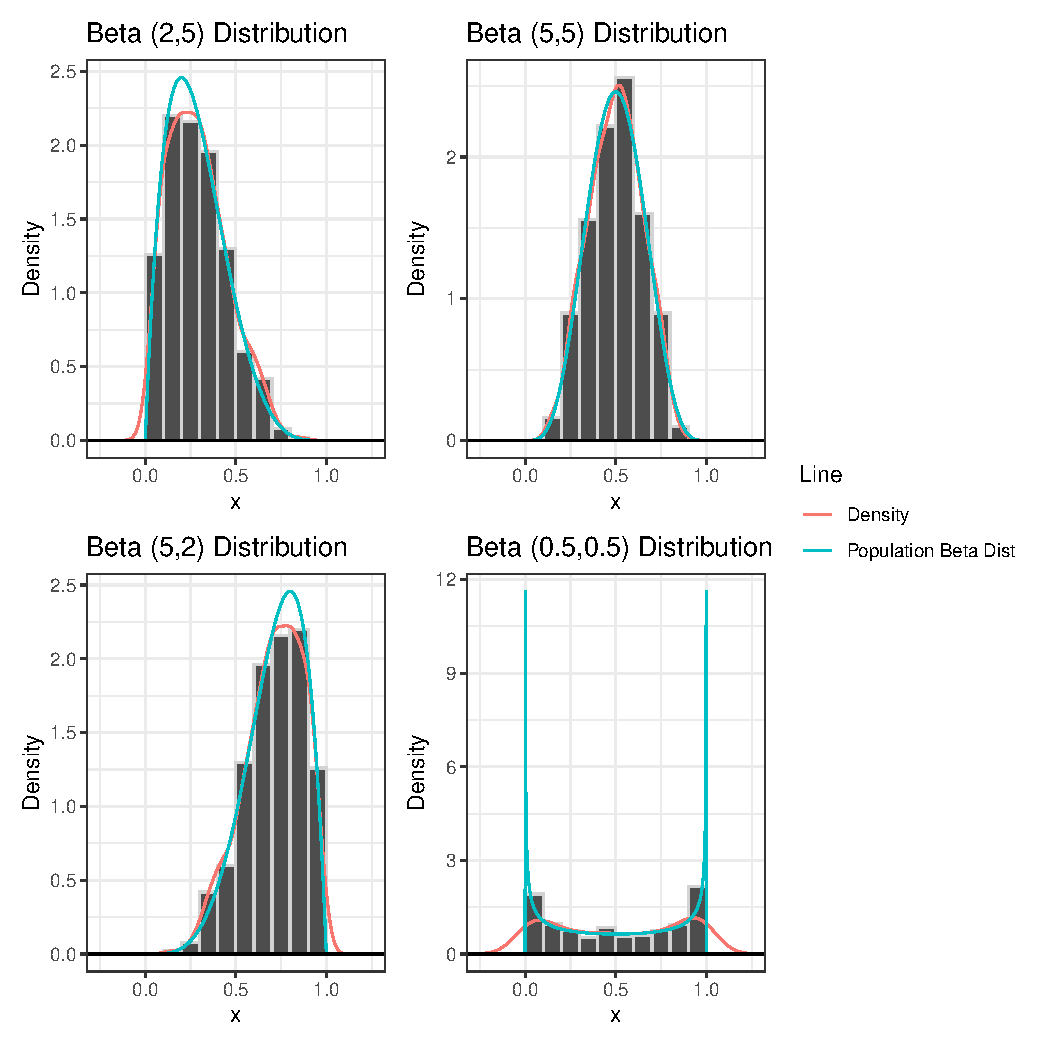
\includegraphics[width=\maxwidth]{figure/plot2-1} 
\end{knitrout}

\begin{figure}[H]
\begin{center}

\caption{Sample Figures for Various Beta Distributions}
\label{samplehistograms} %we can now reference plot1
\end{center}
\end{figure}

\subsection{Estimators}

\subsection{Example}

\end{document}
